\documentclass[journal]{IEEEtran}
% \documentclass[12pt,letterpaper]{article}
\usepackage[margin=1in]{geometry}
\usepackage[english]{babel}
\usepackage[utf8x]{inputenc}
\usepackage{amsmath}
\usepackage{amssymb} 
% \usepackage[retainorgcmds]{IEEEtrantools}
\usepackage{graphicx}
\usepackage{tabularx}
\usepackage{kpfonts}    % for nice fonts
\usepackage{microtype} 
\usepackage{booktabs}   % for nice tables
\usepackage{bm}         % for bold math
\usepackage{listings}   % for inserting code
\usepackage{verbatim}   % useful for program listings
\usepackage{color} 
\usepackage[colorlinks=true]{hyperref}
% use for hypertext
% \usepackage[colorinlistoftodos]{todonotes}
\usepackage{natbib}

\usepackage{xcolor}
\usepackage{subcaption}

\newtheorem{definition}{Definition}
\newtheorem{theorem}{Theorem}
\newtheorem{proposition}{Proposition}
\newtheorem{corollary}{Corollary}
\newtheorem{lemma}{Lemma}
\newtheorem{example}{Example}

\usepackage{lipsum}

\begin{document}

\title{Title for \textit{Project} ECE 227}
        
    \author{
    \IEEEauthorblockN{Author 1},
    \IEEEauthorblockA{\textit{Department of [YOUR DEPARTMENT]} \\
    \textit{UC San Diego}\\
    mail1@mail.com}

    \and
    
    \IEEEauthorblockN{Author 2},
    \IEEEauthorblockA{\textit{Department of [YOUR DEPARTMENT]} \\
    \textit{UC San Diego}\\
    mail2@mail.com}
    \and
    
    \IEEEauthorblockN{Author 3},
    \IEEEauthorblockA{\textit{Department of [YOUR DEPARTMENT]} \\
    \textit{UC San Diego}\\
    mail3@mail.com}
    }
    
\maketitle
%-Title
%+Abstract
\begin{abstract}
\lipsum[1]
\end{abstract}
%-Abstract

\captionsetup{font=footnotesize} % or small


\section{Introduction}
The Prisoner’s Dilemma is a two‐player game in which each participant can either cooperate or defect. The outcomes are either mutual cooperation, yielding a moderate reward for both; unilateral defection, giving the defector a high payoff and the cooperator a low payoff; and mutual defection, leaving both with a low payoff. 

In this paper, we examine the Prisoner's Dilemma’s dynamics on two empirically derived social networks: the Facebook Social Circles (from SNAP) and the Epinions graph (also from SNAP). On each network, we first employ a standard "imitate the best" update rule, whereby each node plays PD with all neighbors, counts payoffs, and then takes the highest payoff neighbor's strategy. Then, on the Epinions network, we suggest a trust‐sensitive version: after each round, agents only consider neighbors that they trust when determining whom to copy.

\section{Related Works}
A substantial body of past research has explored how network structure and trust relationships influence cooperation in an iterative Prisoner’s Dilemma setting. Cameron and Cintrón-Arias revisit the PD on real social networks, demonstrating that empirical topologies, characterized by heterogeneous degree distributions and community structure, play a crucial role in the spread and stability of cooperative strategies. High-degree nodes and clustering sometimes facilitate and sometimes obstruct cooperation, depending on the payoffs and update rules. Dynamic social networks facilitate cooperation in the N-player Prisoner’s Dilemma by Rezaei and Kirley and they build on this by introducing dynamic rewiring in the N-player PD. This allows agents to adjust ties based on past payoffs so that defectors lose links and cooperators attract new ones, which leads to defectors being isolated while cooperators cluster together. Meanwhile, Trust-induced cooperation under the complex interaction of networks and emotions by Xie et al. looks at “trust-induced cooperation” under complex network and emotional interactions by embedding a continuous, weighted trust metric into the agent’s decisions. This stabilized cooperation under harsher payoff conditions and produces more accurate patterns of cooperation compared to real social behavior.

         
\section{Model}
\begin{figure*}[ht]
    \centering
    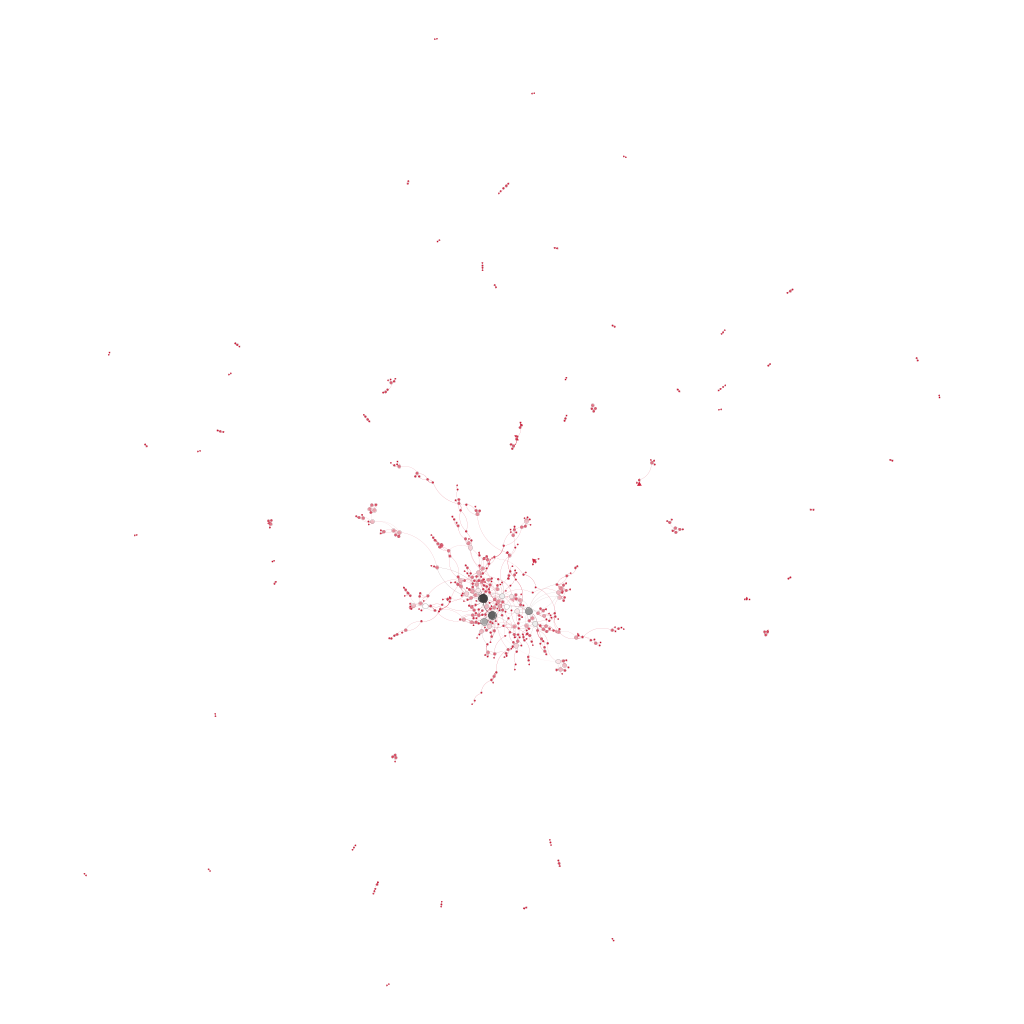
\includegraphics[width=0.3\linewidth]{figures/Calls_network.png}
    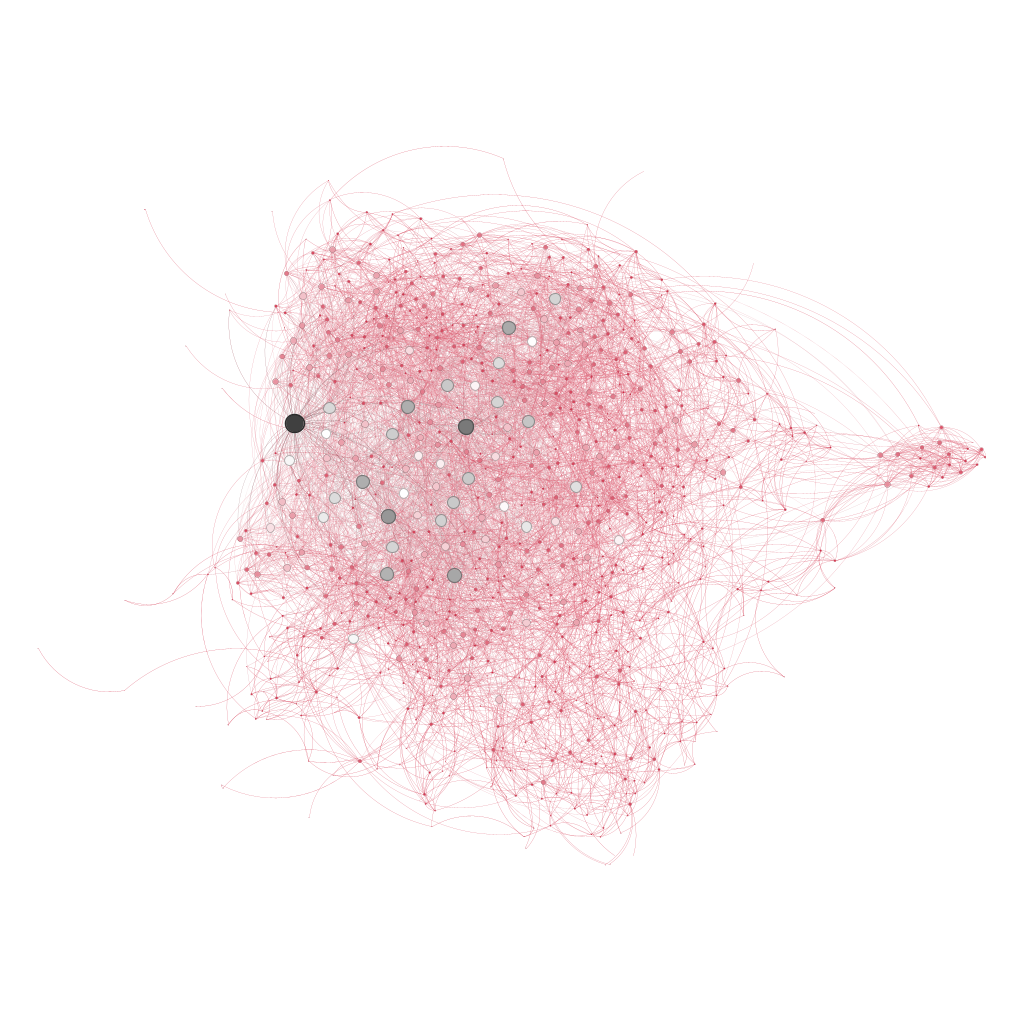
\includegraphics[width=0.3\linewidth]{figures/FB_network.png}
    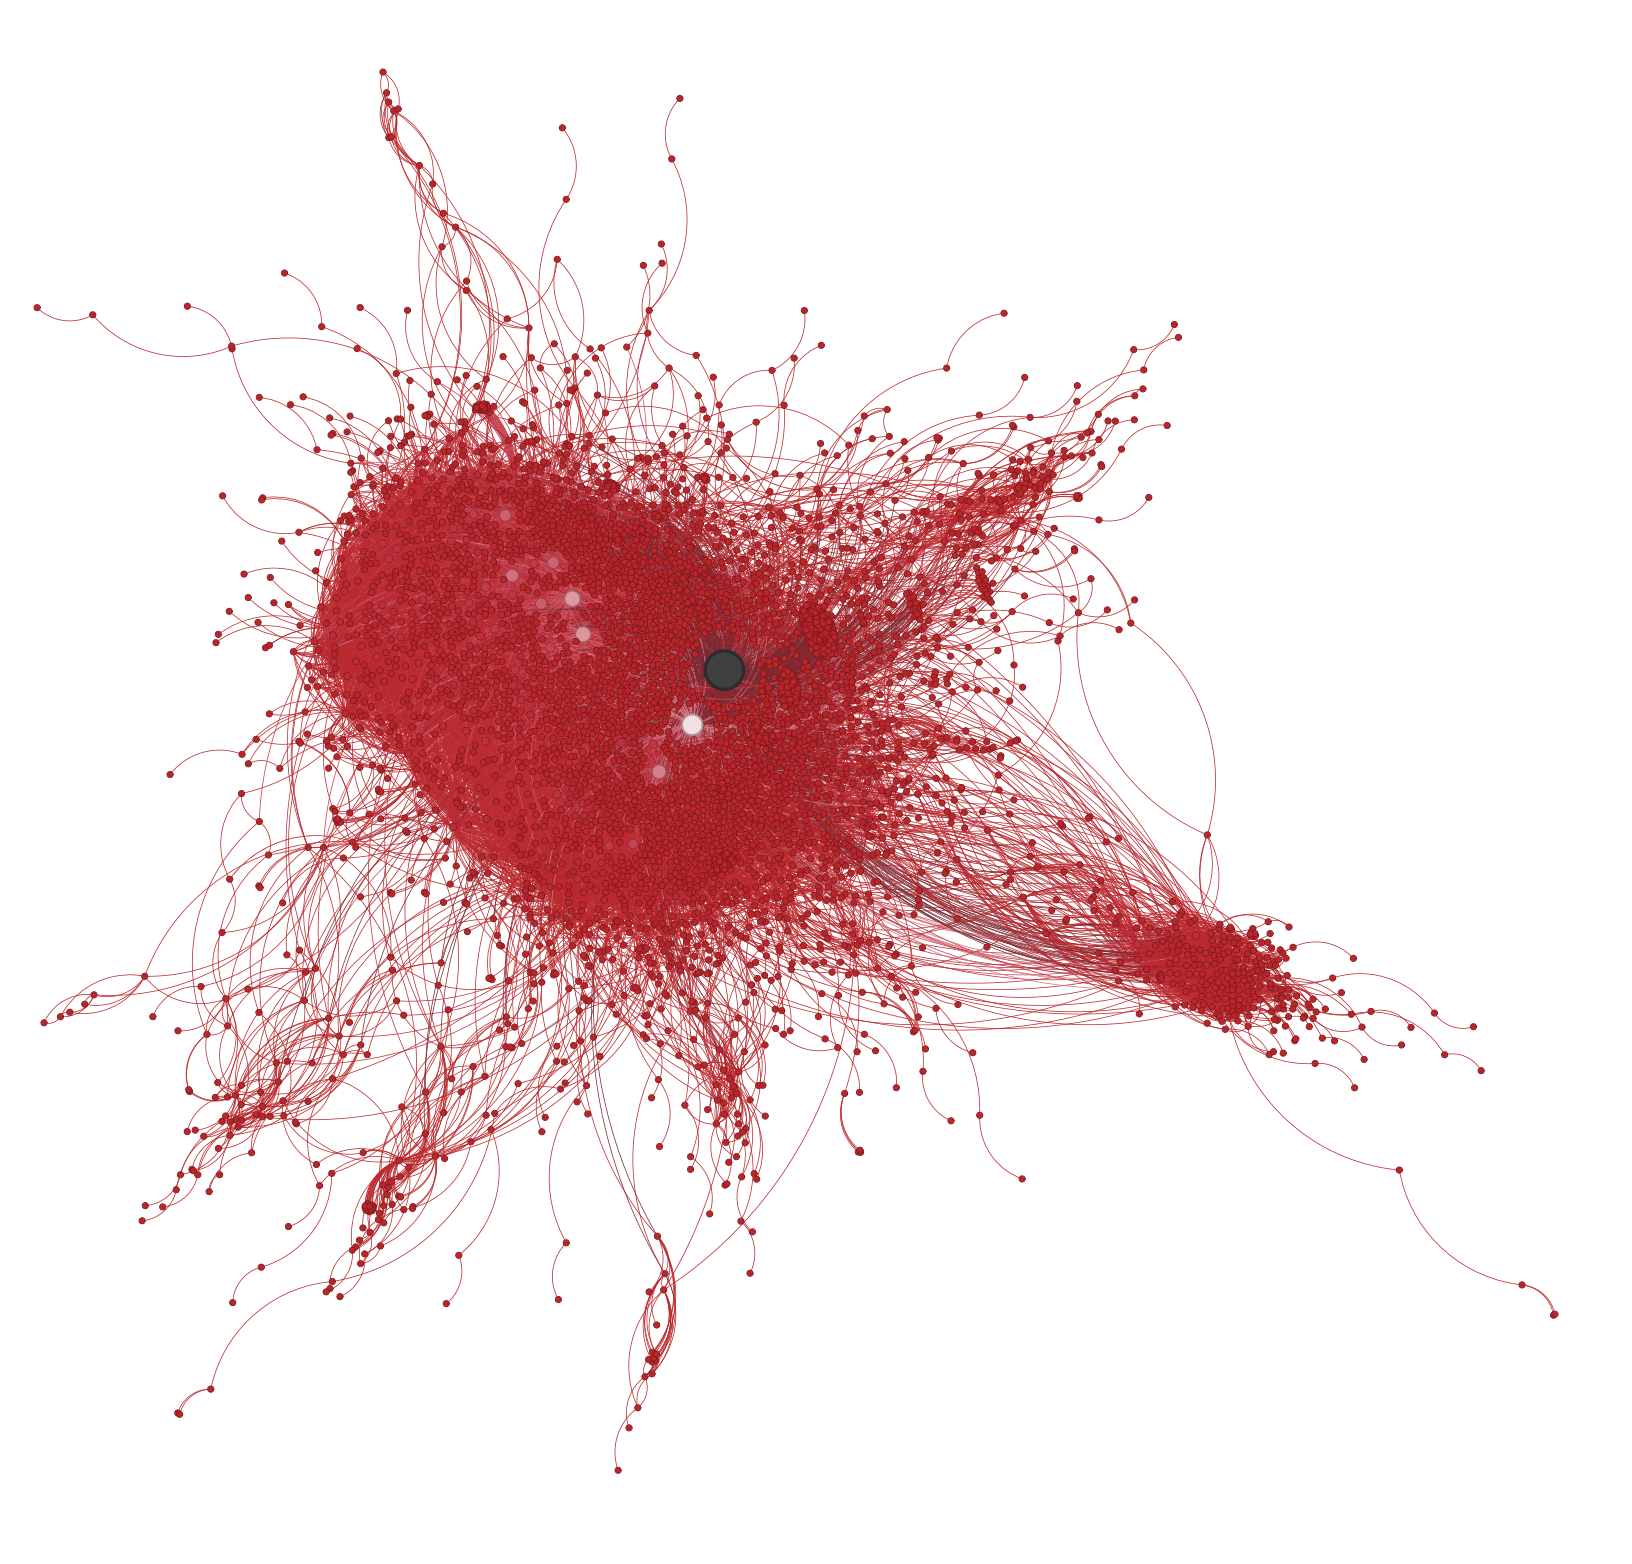
\includegraphics[width=0.3\linewidth]{figures/ff.png}
    \caption{Figure example}
    \label{fig:enter-label}
\end{figure*}


The first network we looked at was the Facebook dataset (SNAP). This network consists of anonymized ego-networks extracted from Facebook, where each node represents a user and edges represent friendship links. Using this as our base, we assigned each node’s initial strategy with a Bernoulli (0.5) distribution, giving an equal chance between cooperation and defection. Then, after every game iteration playing Prisoner’s Dilemma, there is an update strategy where each node will look at all its neighbors and will adopt the more successful strategy. 
The next network we looked at was the Epinions social network dataset (SNAP), a directed “who-trusts-whom” graph from the Epinions.com review site, where each edge indicates that one user has marked another as trusted or not trusted. 

\section{Dataset Description}

The first network we examined was the Facebook “circles” network, which is constructed by aggregating the ego-networks of ten anonymized survey participants, each of whom contributes an “ego” node linked to all their friends. The resulting graph ends up with 4,039 nodes and 88,234 edges, where each edge represents a friend connection. The network is highly connected and strongly clustered, with the average node degree being 43.7 and the cluster coefficient being 0.6055. Furthermore, the network has a small-world nature where the diameter of the network is 8, meaning the longest shortest path between any two users is 8 hops. 

\begin{figure}[ht]
    \centering
    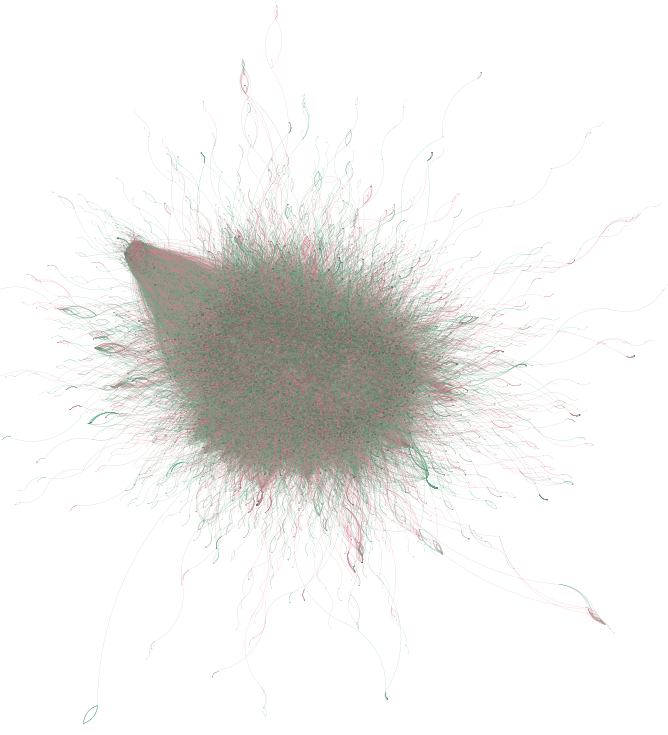
\includegraphics[width=0.8\linewidth]{figures/init_fb.png}
    \caption{Facebook Network}
    \label{fig:enter-label}
\end{figure}

The second network we examined was the Epinions social network, which is a directed graph where each node represents a user on the Epinions.com review website, and each edge will either state whether the user trusts or distrusts another user. The network is comprised of 131,828 nodes and 841,372 edges. Although the entire users form a large strong weakly connected component of 119,130 nodes (90.4\% of the graph) with 833,695 edges (99.1\% of the total). The strongly connected component is relatively small, i.e., just 41,441 users (31.4\%) who mutually trust one another with 693,737 edges (82.5\%). The average clustering coefficient of the network is 0.1279, which indicates moderate local clustering. Lastly, this network also has a small-world nature, with the diameter being 14. 

\begin{figure}[ht]
    \centering
    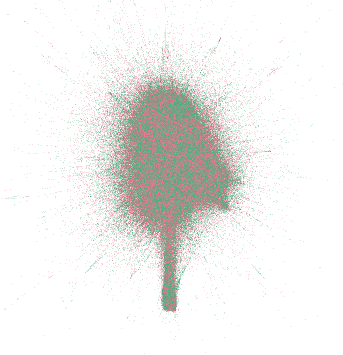
\includegraphics[width=0.8\linewidth]{Project Template for ECE227/figures/init_epinions.png}
    \caption{Epinions Network}
    \label{fig:enter-label}
\end{figure}

\section{Simulations and Numerical Experiments}

We conducted evolutionary Prisoner’s Dilemma simulations on both networks, varying the initial state of Bernoulli for the starting strategies \(p \in \{0.25, 0.50, 0.75\}\). For each combination of network and \(p\), we compared two standard payoff‐based update rules (imitate‐best‐neighbor and Fermi). Then for every combination of the Epinions' data set, we compared the trust update rules (trust aware update and all neighbor trust).  In every experiment, we recorded the final fraction of cooperators and the number of iterations required for the dynamics to converge.


\subsection{Intuition}
Prior to conducting our simulations, we formulated the following expectations. First, we hypothesized that under standard payoff‐based update rules (imitate‐best‐neighbor and Fermi), the dense, highly clustered Facebook network would sustain higher levels of cooperation than the sparser, more hierarchical Epinions network. Second, we expected that introducing trust-awareness into the update process would uniformly boost cooperative behavior. Finally, we expected that an all‐neighbor trust aggregation rule—by leveraging the full spectrum of positive and negative ties—would produce the most robust and rapid convergence to cooperation across both network topologies.


\section{Results}

\subsection{Cooperation Levels}
Table \ref{tab:fb_ep_compact_final} presents the final fraction of cooperators under three initial distribution parameters \(p\) (initial cooperation probability) for both the Facebook and Epinions networks across four update rules. 
Under standard \emph{imitate‐best‐neighbor} and game, Facebook converges to 0\% cooperation at \(p=0.25\) and to 95.8\% at \(p=0.75\), whereas Epinions peaks at 27.4\% cooperation when \(p=0.75\). 
This shows that for both the Facebook and Epinions networks, cooperation is highly sensitive to the initial cooperation distributions under the \emph{imitate‐best‐neighbor} update rule. 
It is also likely that there exists a critical \(p\) for the Facebook network that determines whether it will converge to majority cooperate or defect.

The Fermi rule yields vastly different behavior: Facebook reaches only 5.94\% cooperation at high \(p\), while Epinions remains below 31\%. 
In both networks, the Fermi update rule leads to a more gradual increase in cooperation as \(p\) increases, with Facebook showing a slight increase from 1.51\% at \(p=0.25\) to 5.94\% at \(p=0.75\), while Epinions shows a similar trend from 8.05\% to 30.47\%.

When we apply both imitation and Fermi updates on Epinions with the trust-aware game, final cooperation rises sharply into the 62–82\% range across all \(p\). 
Unlike the standard game, the results of the trust-aware game show that cooperation is less sensitive to the initial distribution \(p\) and update rule, with all three \(p\) values yielding similar final cooperation levels.
The \emph{trust-aware update} rule achieves 9.32\% cooperation at \(p=0.25\) and 31.5\% at \(p=0.75\), while the \emph{all-neighbor-trust} rule drives cooperation above 90\% across all \(p\) values, demonstrating the power of trust in greatly enhancing cooperation.
These cooperation results indicate that trust-aware updates generally outperform standard imitation and \emph{Fermi} updates, especially in the sparse Epinions network.


\subsection{Convergence Speed}
Table \ref{tab:fb_ep_compact_final} also presents the the number of iterations taken for each update rule to reach equilibrium with a tolerance of 0.05\%.
Under the standard game with the \emph{imitate‐best‐neighbor} update rule, Facebook converges in 3 iterations at \(p=0.25\) and 5 iterations at both \(p=0.50\) and \(p=0.75\).
On Epinions, the same rule requires 4, 6, and 8 iterations respectively, indicating that the sparse topology of Epinions leads to slower convergence compared to Facebook.
The \emph{Fermi} update rule exhibits a similar pattern; Facebook takes 10, 7, and 17 iterations at \(p=0.25\), \(p=0.50\), and \(p=0.75\) respectively, 
while Epinions requires 9, 16, and 20 iterations. However, the \emph{Fermi} update rule is generally slower to converge as can be seen in the exponential shape of the convergence curves in the plots.
The introduction of trust awareness significantly affects convergence on Epinions. 
The trust update rules including both pairwise trust updates and the \emph{all‐neighbor‐trust} converge in under 10 iterations (often within 5–8), highlighting trust’s ability to accelerate consensus.
Thus, trust-aware mechanisms consistently accelerate convergence, reaching equilibrium in fewer iterations than standard imitation or \emph{Fermi} update rules, regardless of initial conditions.


\begin{landscape}
\begin{table}[p]
  \centering
  % Use the smallest readable font:
  \tiny
  \caption{“Cooperator (\%) vs.\ Iteration” plots, final‐split percentages, and iterations to convergence, organized by update rule.}
  \label{tab:fb_ep_compact_final}
  \vspace{0.5em}

  % Define a very narrow column type “S” for Final‐Split cells
  \newcolumntype{S}{>{\centering\arraybackslash}m{0.8cm}}
  % Define a very wide column type “P” for plot cells
  \newcolumntype{P}{>{\centering\arraybackslash}m{4.2cm}}

  % Tighten spacing between columns
  \setlength{\tabcolsep}{2pt}

  % Define the new, mixed table structure: S-S-S-P for FB, P-S-S-S for EP
  \begin{tabular}{%
      l | S S S P | P S S S | P S S S
    }
    \toprule
    % Row 1: Dataset
    & \multicolumn{4}{c|}{\bfseries Facebook}
    & \multicolumn{8}{c}{\bfseries Epinion} \\
    \cmidrule(lr){2-5} \cmidrule(lr){6-13}

    % Row 2: Game Type
    {\bfseries Update Rule}
    & \multicolumn{4}{c|}{\bfseries Std. Game}
    & \multicolumn{4}{c|}{\bfseries Std. Game}
    & \multicolumn{4}{c}{\bfseries Trust-Aware} \\
    \cmidrule(lr){2-5} \cmidrule(lr){6-9} \cmidrule(lr){10-13}

    % Row 3: Header for split percentages and convergence iterations
    & \multicolumn{3}{c|}{\bfseries\shortstack{Cooperate \% \\[-0.3em] Defect \% \\[-0.3em] (Conv. Iter.)}} & {\bfseries Plot}
    & {\bfseries Plot} & \multicolumn{3}{c|}{\bfseries\shortstack{Cooperate \% \\[-0.3em] Defect \% \\[-0.3em] (Conv. Iter.)}}
    & {\bfseries Plot} & \multicolumn{3}{c}{\bfseries\shortstack{Cooperate \% \\[-0.3em] Defect \% \\[-0.3em] (Conv. Iter.)}} \\
    \cmidrule(lr){2-4} \cmidrule(lr){7-9} \cmidrule(lr){11-13}

    % Row 4: p-values
    & {\(p=0.25\)} & {\(p=0.50\)} & {\(p=0.75\)} &
    & & {\(p=0.25\)} & {\(p=0.50\)} & {\(p=0.75\)}
    & & {\(p=0.25\)} & {\(p=0.50\)} & {\(p=0.75\)} \\
    \midrule

    Imitate–Best–Neighbor
      % Facebook Std. Game (S-S-S-P)
      & \shortstack{0.00\%\\100.00\%\\(3)} & \shortstack{77.25\%\\22.75\%\\(5)} & \shortstack{95.79\%\\4.21\%\\(5)}
      & 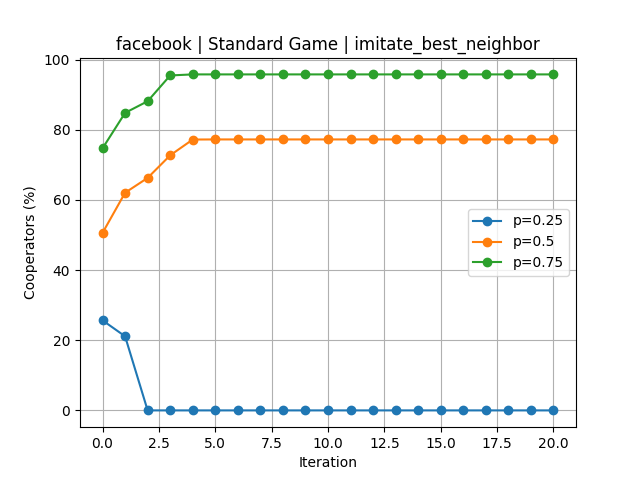
\includegraphics[width=4cm]{figures/plots/facebook_evolutionary_game_round_imitate_best_neighbor.png}
      % Epinion Std. Game (P-S-S-S)
      & 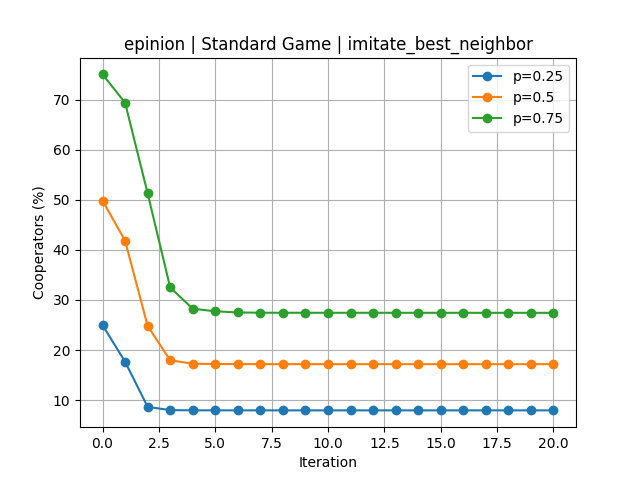
\includegraphics[width=4cm]{figures/plots/epinion_evolutionary_game_round_imitate_best_neighbor.png}
      & \shortstack{7.95\%\\92.05\%\\(4)} & \shortstack{17.18\%\\82.82\%\\(6)} & \shortstack{27.43\%\\72.57\%\\(8)}
      % Epinion Trust-Aware Game (P-S-S-S)
      & 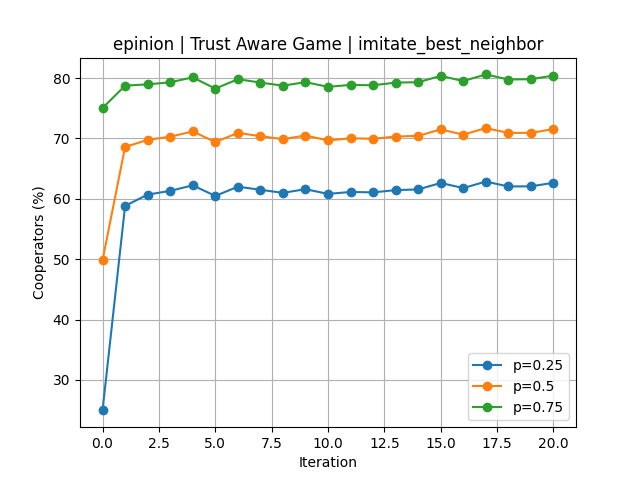
\includegraphics[width=4cm]{figures/plots/epinion_game_round_trust_imitate_best_neighbor.png}
      & \shortstack{62.66\%\\37.34\%\\(19)} & \shortstack{71.55\%\\28.45\%\\(19)} & \shortstack{80.42\%\\19.58\%\\(20)}
      \\[0.6em]

    Fermi–Update
      % Facebook Std. Game (S-S-S-P)
      & \shortstack{1.51\%\\98.49\%\\(10)} & \shortstack{5.89\%\\94.11\%\\(7)} & \shortstack{5.94\%\\94.06\%\\(17)}
      & 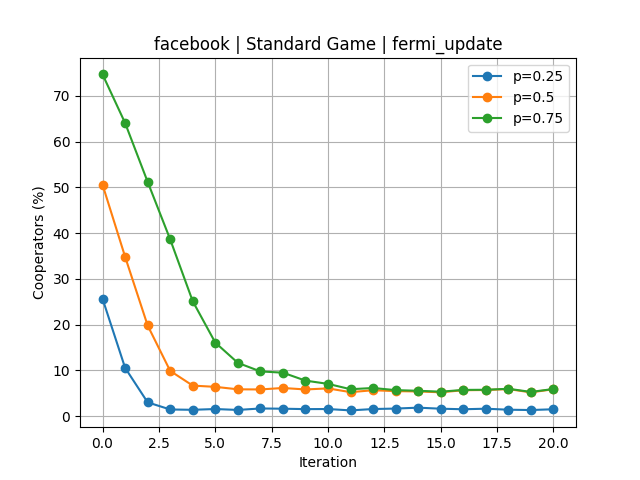
\includegraphics[width=4cm]{figures/plots/facebook_evolutionary_game_round_fermi_update.png}
      % Epinion Std. Game (P-S-S-S)
      & 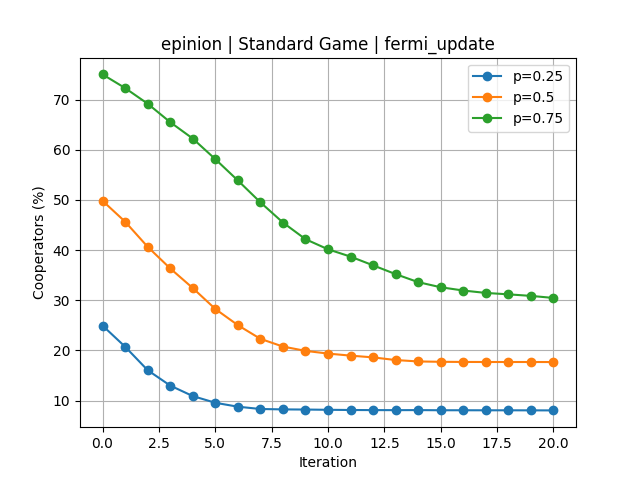
\includegraphics[width=4cm]{figures/plots/epinion_evolutionary_game_round_fermi_update.png}
      & \shortstack{8.05\%\\91.95\%\\(9)} & \shortstack{17.69\%\\82.31\%\\(16)} & \shortstack{30.47\%\\69.53\%\\(20)}
      % Epinion Trust-Aware Game (P-S-S-S)
      & 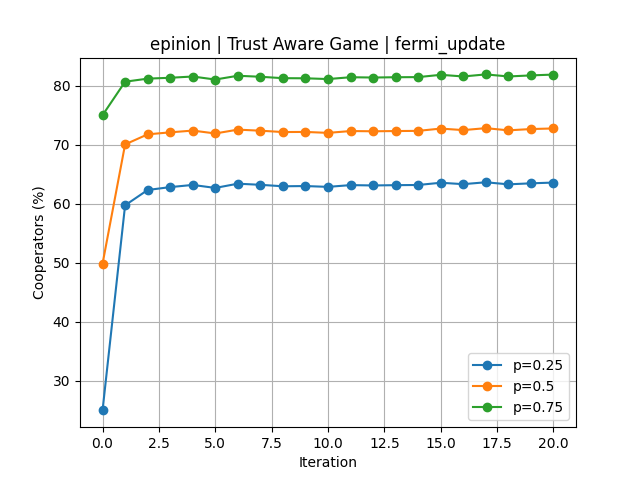
\includegraphics[width=4cm]{figures/plots/epinion_game_round_trust_fermi_update.png}
      & \shortstack{63.61\%\\36.39\%\\(9)} & \shortstack{72.79\%\\27.21\%\\(9)} & \shortstack{81.93\%\\18.07\%\\(9)}
      \\[0.6em]

    Trust–Aware–Update
      % Facebook Std. Game (N/A, S-S-S-P)
      & \shortstack{N/A\\N/A\\N/A} & \shortstack{N/A\\N/A\\N/A} & \shortstack{N/A\\N/A\\N/A}
      & \shortstack{N/A}
      % Epinion Std. Game (P-S-S-S)
      & 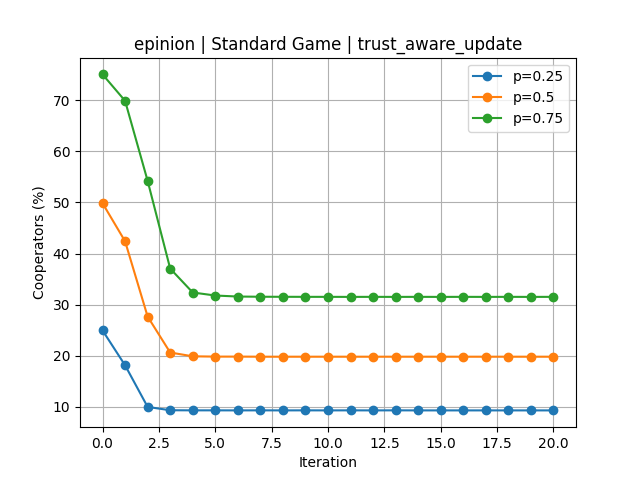
\includegraphics[width=4cm]{figures/plots/epinion_evolutionary_game_round_trust_aware_update.png}
      & \shortstack{9.32\%\\90.68\%\\(4)} & \shortstack{19.82\%\\80.18\%\\(6)} & \shortstack{31.53\%\\68.47\%\\(7)}
      % Epinion Trust-Aware Game (P-S-S-S)
      & 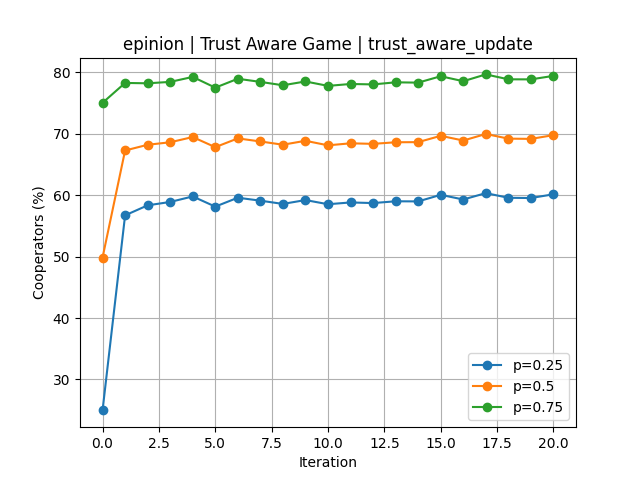
\includegraphics[width=4cm]{figures/plots/epinion_game_round_trust_trust_aware_update.png}
      & \shortstack{60.15\%\\39.85\%\\(14)} & \shortstack{69.78\%\\30.22\%\\(14)} & \shortstack{79.43\%\\20.57\%\\(14)}
      \\[0.6em]

    All–Neighbor–Trust
      % Facebook Std. Game (N/A, S-S-S-P)
      & \shortstack{N/A\\N/A\\N/A} & \shortstack{N/A\\N/A\\N/A} & \shortstack{N/A\\N/A\\N/A}
      & \shortstack{N/A}
      % Epinion Std. Game (P-S-S-S)
      & 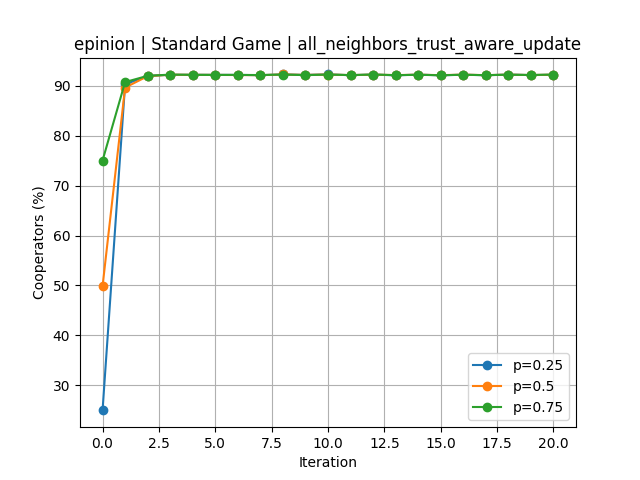
\includegraphics[width=4cm]{figures/plots/epinion_evolutionary_game_round_all_neighbors_trust_aware_update.png}
      & \shortstack{92.24\%\\7.76\%\\(4)} & \shortstack{92.25\%\\7.75\%\\(4)} & \shortstack{92.27\%\\7.73\%\\(4)}
      % Epinion Trust-Aware Game (P-S-S-S)
      & 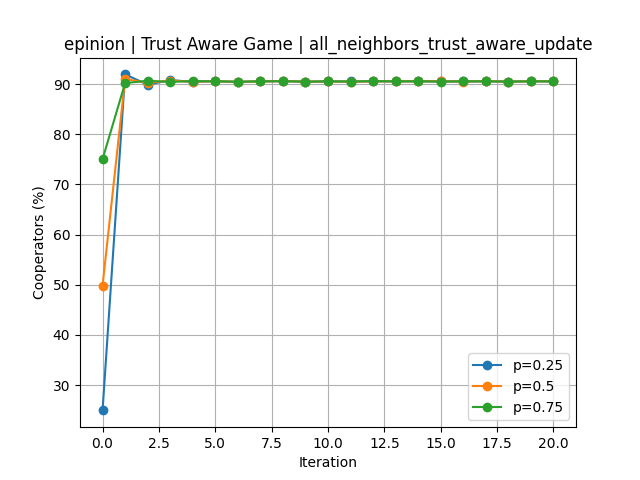
\includegraphics[width=4cm]{figures/plots/epinion_game_round_trust_all_neighbors_trust_aware_update.png}
      & \shortstack{90.54\%\\9.46\%\\(8)} & \shortstack{90.57\%\\9.43\%\\(8)} & \shortstack{90.57\%\\9.43\%\\(7)}
      \\

    \bottomrule
  \end{tabular}
\end{table}
\end{landscape}
\section{Conclusion}
\lipsum[13]

\section{Future works}
\lipsum[14]

\clearpage
\bibliographystyle{apalike}
\bibliography{aguiar}

\newpage

\begin{IEEEbiography}[{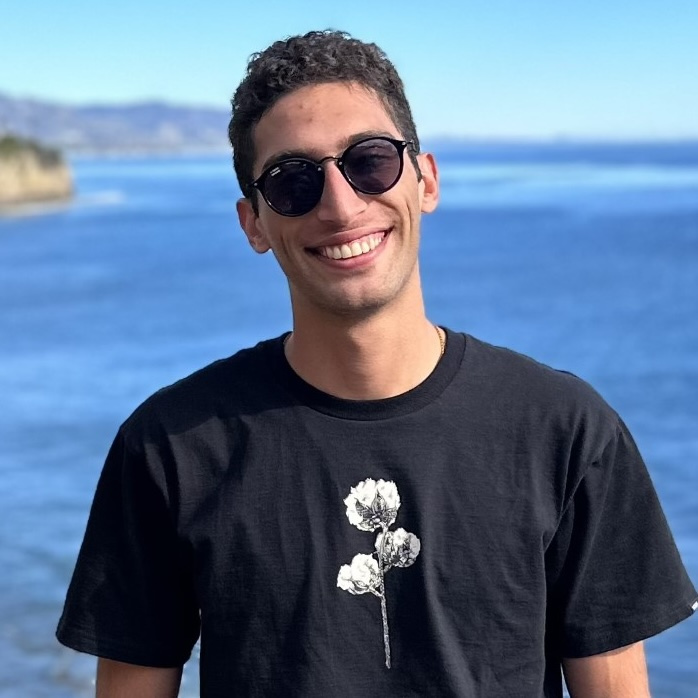
\includegraphics[width=1in,height=1.25in,clip,keepaspectratio]{figures/raman.jpg}}]{Raman Ebrahimi} earned his B.Sc. degrees in Physics and Industrial Engineering from Sharif University of Technology in 2022. His thesis was on the spread of (Dis)Information over the Networks. He received his M.S. degree in March 2025 and his thesis, titled ``From Games to Predictions: Strategic Behavior in Networks and Classification'' focused on applications of game theory and network science in modeling agent behavior. He is now working towards his Ph.D. in Electrical and Computer Engineering at the University of California, San Diego with a special focus on machine learning and data science. His research focuses on game theory, network economics, games on networks, and computational social science. 
\end{IEEEbiography}
\vspace{-1in}
\begin{IEEEbiography}[{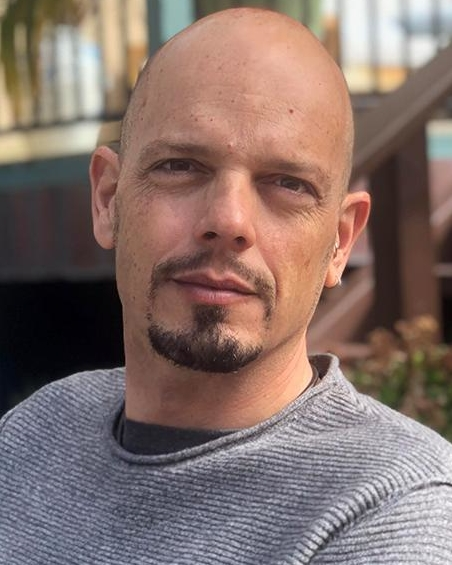
\includegraphics[width=1in,height=1.25in,clip,keepaspectratio]{figures/massimo.jpg}}] {Massimo Franceschetti} graduated in computer engineering from the University of Naples in 1997. He received M.S. and Ph.D. degrees in electrical engineering from the California Institute of Technology in 1999, and 2003 respectively. His doctoral thesis, entitled ``Wireless Networks, from Collective Behavior to the Physics of Propagation'' was awarded the Wilts Prize for best thesis in electrical engineering at Caltech in 2003. He also received the 2000 Walker von Brimer award for outstanding research at Caltech. Franceschetti has held visiting positions at the Vrije Universiteit Amsterdam in the Netherlands, the Ecole Polytechnique Federale de Lausanne in Switzerland, and the University of Trento in Italy. Before joining UCSD, he was a post-doctoral scholar at University of California at Berkeley for two years. 
\end{IEEEbiography}

\end{document}